\section{A simulated example from healthcare}
\label{sec:example}

Given the results in \cref{sec:real_example}, natural questions arise. For example, are such conclusion reversals specific to the explained component? Are these reversals always consequences of model misspecification or sampling variability? Here, we present a simulated example inspired by real-life healthcare data. Our example exhibits sign reversals in the \emph{unexplained} component of the OBD under correct model specification and large sample sizes.

% To illustrate why \cref{eq:ob_decomp_ref_group} can lead a practitioner to draw substantially different conclusions depending on the reference group used in the OBD, we turn to a simple simulated healthcare example inspired by real-life data.

\textbf{Motivation.}
While our example is purely simulated, it is motivated by the following real-life concerns and observations.
Body mass index (BMI) is a widely recognized and routinely measured marker of wellness \cite{heymsfield2016} and is strongly linked to cardiometabolic outcomes, such as elevated blood pressure. 
An important public health question is whether differences in blood pressure between two populations are due mainly to differences in underlying BMI distributions or to differences in how BMI impacts blood pressure \textcolor{red}{can we cite?}.

Our example imagines two populations of adults in primary care being followed for elevated blood pressure, using systolic blood pressure (SBP) at a standardized follow-up visit as the outcome $Y$. The BMI ($X$) of each adult is measured at an initial intake visit.
The first population, Group $H$, comes from a higher-resource setting, such as an urban neighborhood with structured care pathways, frequent follow up, and better access to healthy food and physical activity options. 
The second population, Group $K$, comes from lower-resource setting, where patients face barriers such as longer travel distances to clinics, infrequent follow up, delayed medication titration, and limited access to nutritious food.
These factors shape both the composition of each group (including average BMI) and the structure of the SBP--BMI relationship. We follow a clinical literature finding an approximately linear relationship between BMI and SBP \cite{kaufman1997, cappuccio2008, chen2023}; in particular, we assume a separate linear relationship in each group.

While an OBD cannot establish causality without further assumptions, it can suggest where one might look for potential drivers of observed disparities between the two groups.
If the unexplained component is larger (differences in $Y|X$ dominate), it may highlight the need to investigate differences in medical care, such as medication titration practices, adherence support, or access to antihypertensives. \textcolor{red}{right now we're highlighting a decision that is not a sign-based decision, so that choice clashes with the rest of the narrative}
%In either case, OBD serves only as a descriptive tool that helps formulate hypotheses about where meaningful differences may arise, not as a causal model.
%The answer can inform where to direct limited resources. 
If the explained component is larger (differences in $X$ dominate), targeted interventions on weight management, nutrition, and physical activity may be most impactful. 
%If the unexplained component dominates, changes to care delivery, such as earlier medication titration, improved medication adherence support, or broader access to antihypertensives, may be more effective. 

\textbf{Simulated data.}
We generate the BMI ($X$, in kg/m$^2$) of an individual in group \( g \) from a group-specific normal distribution.
We generate the SBP ($Y$, in mmHg) of an individual in group \( g \) as a noisy function of their BMI:
\begin{equation}
    \label{eq:linear_model}
   Y = \alpha_g + \beta_g \times X + \varepsilon.
\end{equation}
Here $\alpha_g \in \mathbb{R}$ is the group-specific intercept (in units of mmHg); $\beta_g \in \mathbb{R}$ is the group-specific slope, representing the average change in SBP (mmHg) per unit increase in BMI (kg/m$^2$); and $\varepsilon$ reflects individual variability in SBP that is uncorrelated with BMI. We take $\varepsilon$ independent and identically distributed across adult patients, with the same (mean-zero Gaussian) distribution in each group.
We present key parameters in \cref{tab:dgp_short} and provide further details about the data-generating process in \cref{appendix:dgp}.

\begin{table}[h]
\caption{Key chosen and derived parameters by group.}
\label{tab:dgp_short}
\begin{center}
\small
\begin{tabular}{lcccc}
\textbf{Group} & \textbf{Mean BMI} & \textbf{$\alpha$} & \textbf{$\beta$} & \textbf{Mean SBP} \\
\hline \\
H & 25.0 & 110.4 & 1.0 & 135.4 \\
K & 27.0 & 100.0 & 1.4 & 137.8 \\
\end{tabular}
\end{center}
\footnotesize{Note: H = Higher-resource group, K = Lower-resource group. BMI and SBP in kg/m$^2$ and mmHg respectively. $\alpha$ in mmHg, $\beta$ in mmHg per kg/m$^2$.}
\end{table}

\cref{fig:bmi_sbp} shows the fitted BMI–SBP relationships for both groups, showing how differences in intercepts, slopes, and BMI distributions interact.

\begin{figure}[h]
\centerline{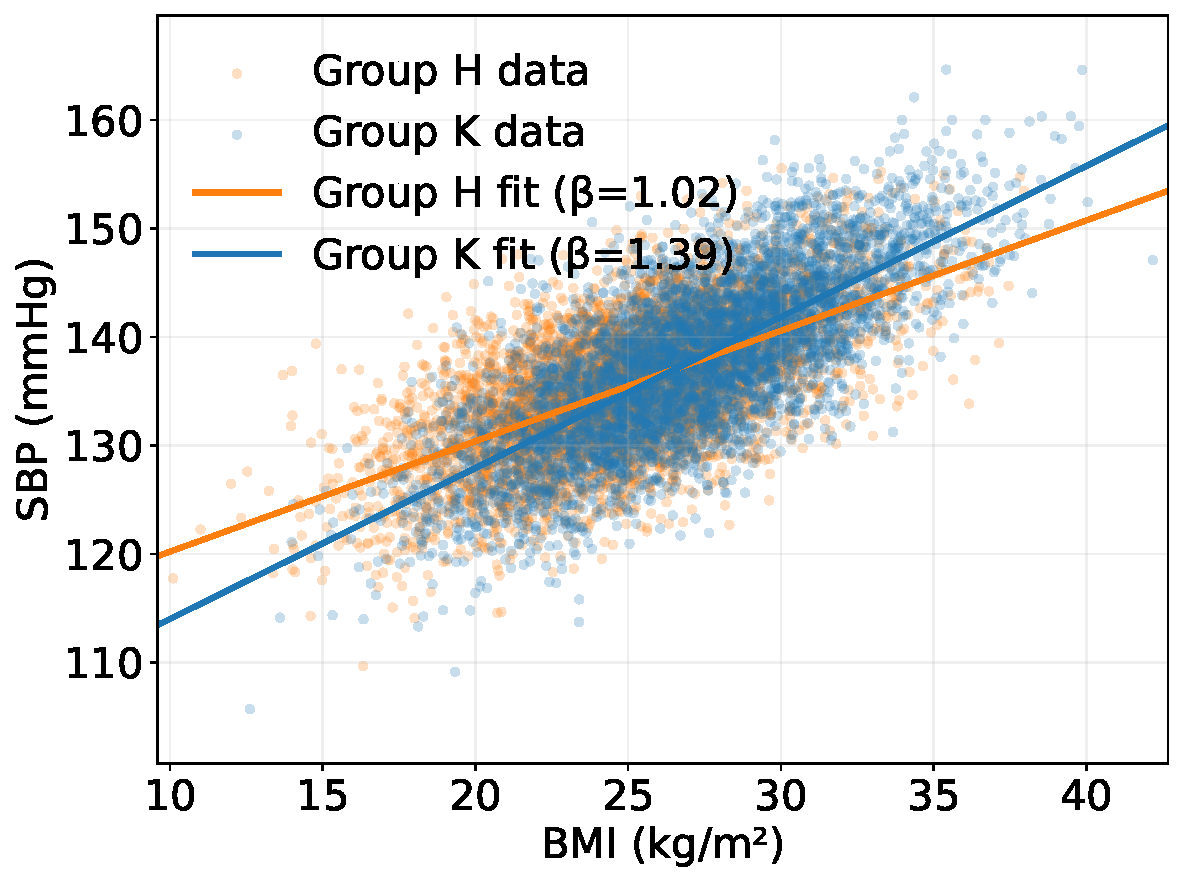
\includegraphics[width=0.75\linewidth]{Sections/Figures/bmi_sbp_comparison.pdf}}
\caption{Fitted linear models of SBP on BMI by group.}
\label{fig:bmi_sbp}
\end{figure}

Analogous to the real-case study in \cref{sec:real_example}, the two fitted lines display a similar qualitative pattern. Overall, Group $H$ has lower average SBP than Group $K$, owing both to lower average BMI and a shallower slope relating BMI to SBP, perhaps reflecting improved access and adherence to treatment, or availability of non-pharmacological support.
However, Group $H$ has a higher baseline SBP ($\alpha_H$), perhaps reflecting genetic factors in Group $H$.

In principle, the OBD should provide a transparent framework to separate the difference in mean SBP into an explained component (differences in BMI distribution, $X$) and an unexplained component (differences in SBP given BMI, $Y|X$)
\cref{tab:ob_decomp} summarizes the OBD results, taking $H$ and $K$ as the reference groups in turn.

\begin{table}[H]
\caption{Estimated Oaxaca–Blinder decomposition of mean SBP differences}
\label{tab:ob_decomp}
\begin{center}
\small
\begin{tabular}{lrrr}
\textbf{Group} & \textbf{Explained} & \textbf{Unexplained} & \textbf{Total gap} \\
\hline \\
H & $-1.91$ & $\textbf{-0.14}$ & $-2.05$ \\
K & $-2.61$ & $\textbf{0.57}$  & $-2.05$ \\
\end{tabular}
\end{center}
\footnotesize{Note: H = Higher-resource group, K = Lower-resource group. All values in mmHg.}
\end{table}

\begin{figure*}[t]
\vspace{.3in}
\centerline{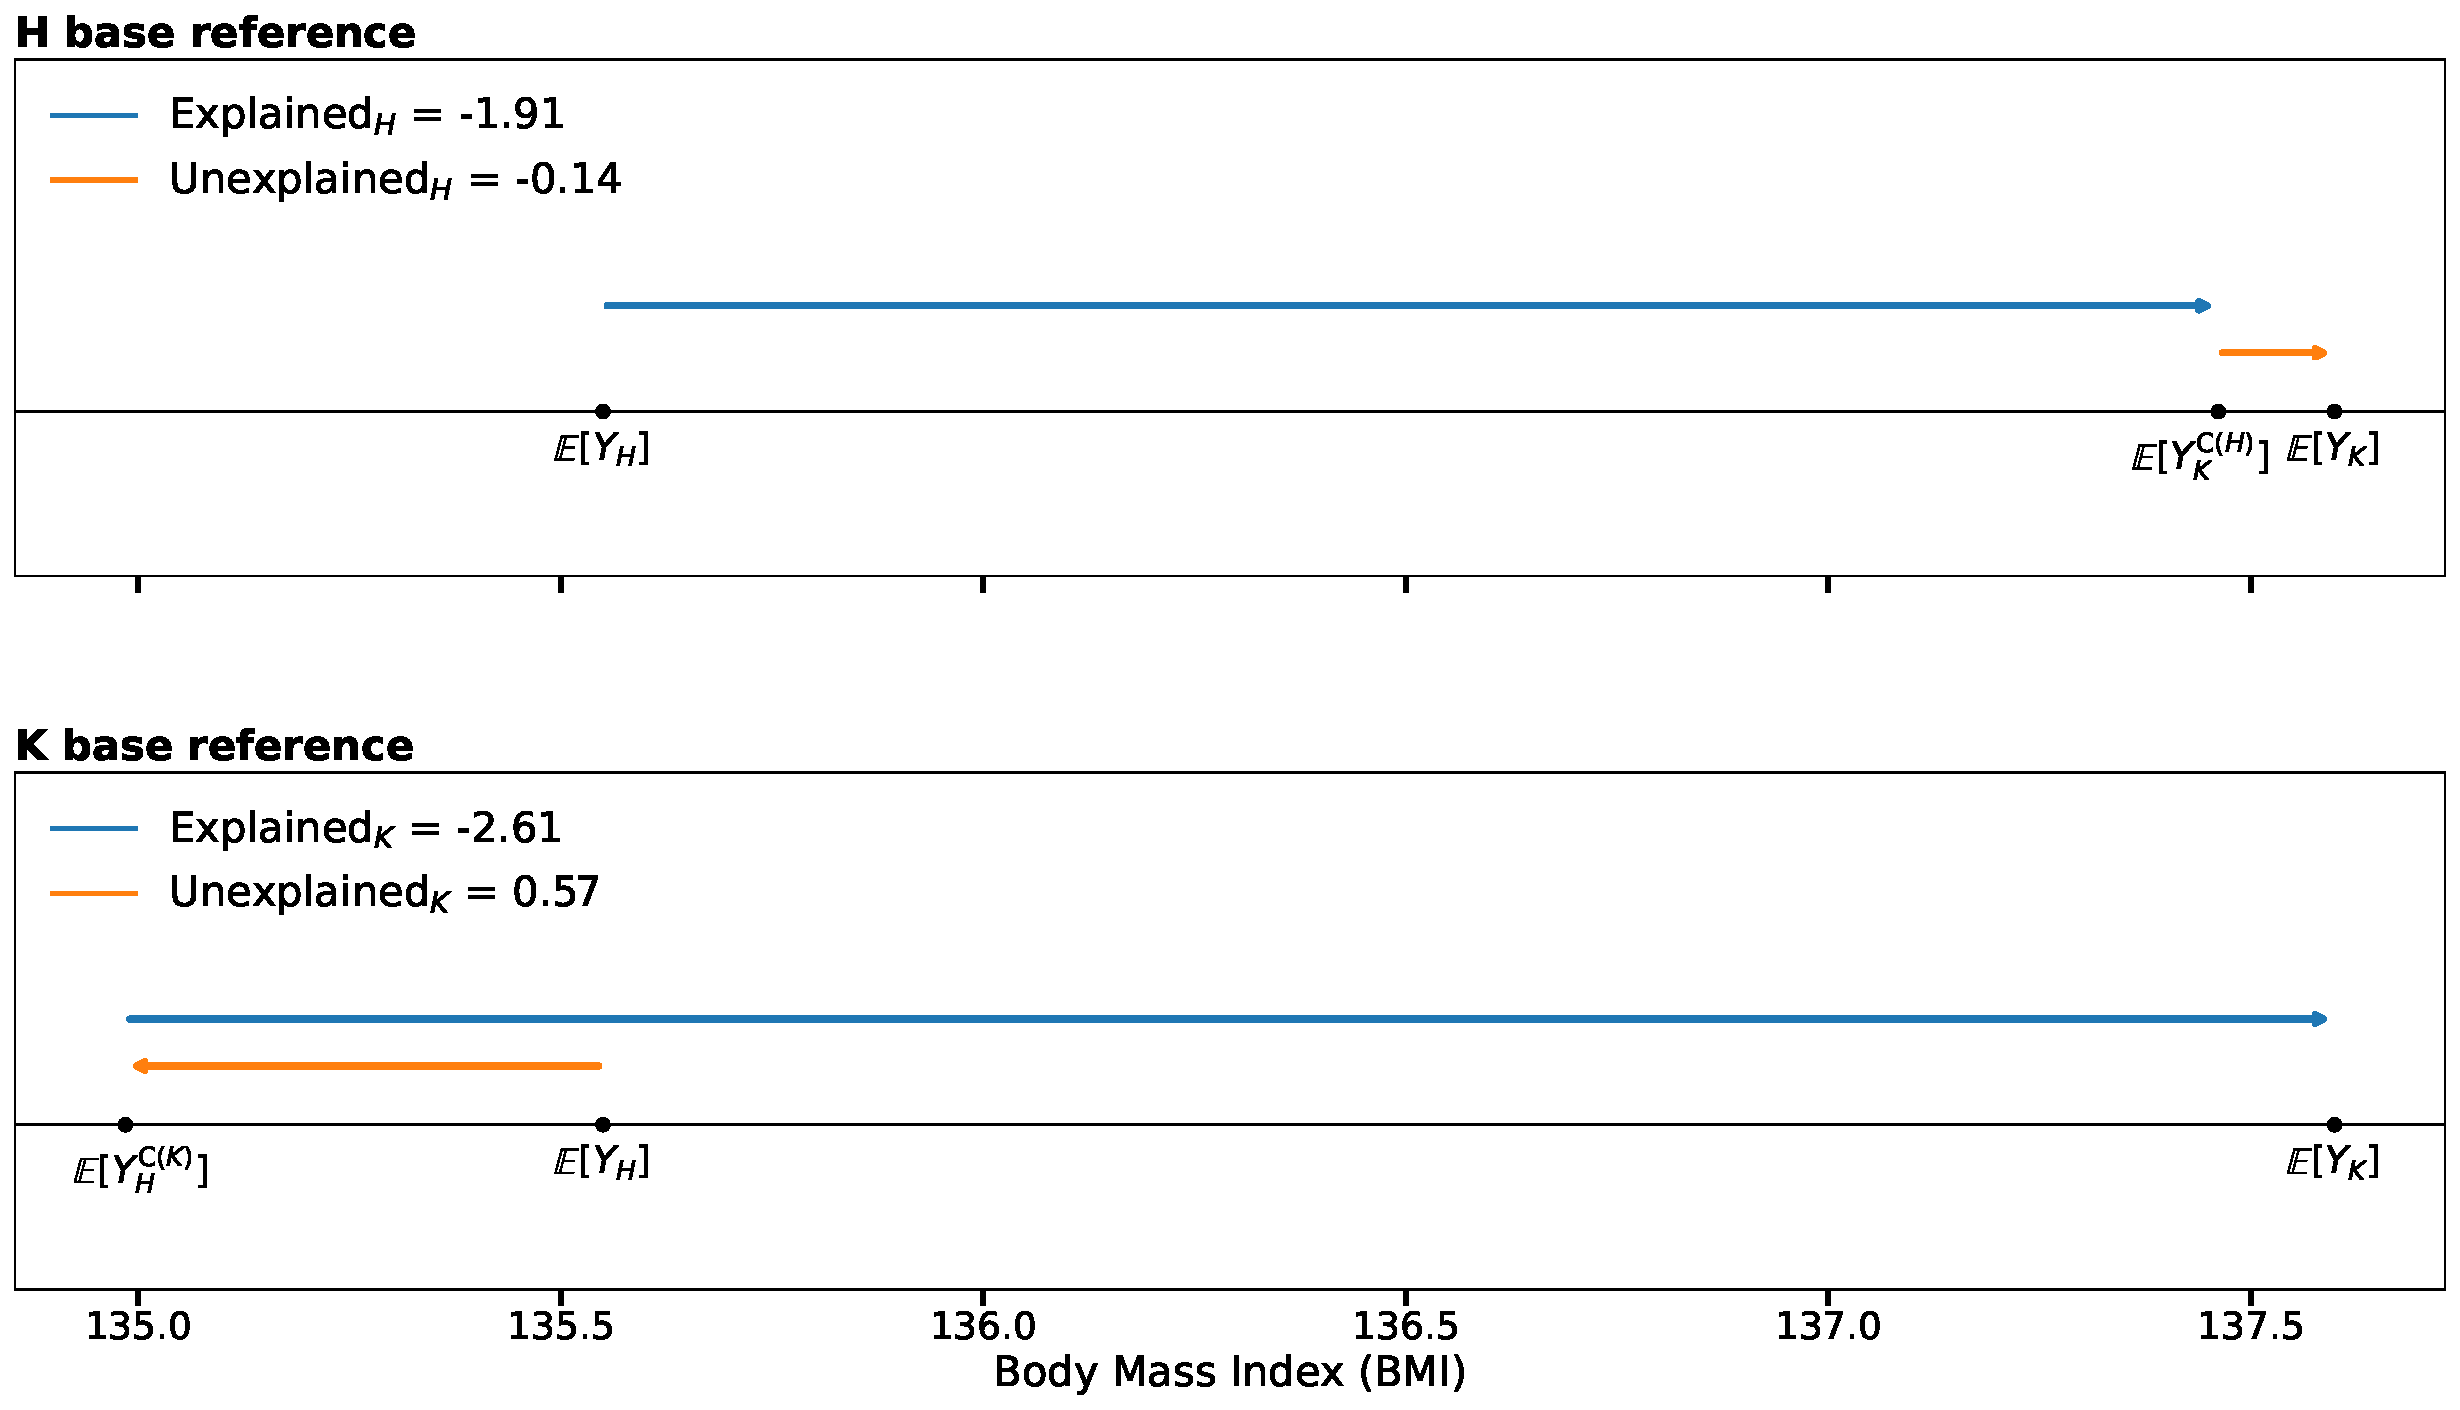
\includegraphics[width=0.7\textwidth]{Sections/Figures/counterfactual.pdf}}
\vspace{.3in}
\caption{Counterfactual analysis visualization showing the decomposition results for both reference groups in our simulated example.}
\label{fig:counterfactual}
\end{figure*}

\cref{fig:counterfactual} visualizes the OBD as the mere difference between the counterfactual question posed by each choice of reference group and the observed mean SBP for each group. It also illustrates the sign flip in the unexplained component.

For both choices of reference group, the explained components are negative, so both choices of reference dsitribution attribute Group $H$'s lower average SBP in part to its lower average BMI.
However, the sign of the unexplained OB component flips depending on the choice of the reference group.
When Group $H$ is the reference, the negative unexplained component implies that institutional factors further reduce Group H's blood pressure.
However, when Group $K$ is the reference, institutional factors appear to \emph{increase} Group $H$'s average blood pressure!
Intuitively, because blood pressure in Group $K$ is so much more responsive to BMI, Group $H$'s lower average BMI appears so good as to ``over-explain'' the difference in SBP; the unexplained component is then forced to be positive to compensate.
Given that the choice of reference distribution is arbitrary here, we conclude that the OBD is not reliable for decomposing differences in this example.

% \textcolor{red}{mega double check conclusion:}
% Some authors might argue that the choice of reference group simply reflects a different counterfactual question, for example, ``What would the SBP gap be if the lower resource group had the BMI--SBP relationship of the higher resource group?'' versus ``What would the gap be if the higher resource group had the BMI--SBP relationship of the lower resource group?'' 
% Others might claim that the true effect lies somewhere between these two extremes, and that averaging across reference groups provides a balanced view. 
% However, in our setting we argue that such sensitivity is problematic: when the sign of the unexplained component reverses, the qualitative policy message changes, creating a real risk of misinterpretation rather than a benign difference in framing.


